% !TeX encoding=utf8
% !TeX spellcheck=de-DE
% !TeX root=../UID_Project_Documentation.tex

\section{Observation}

\subsection{Marktanalyse}

Das Produkt befindet sich im Marktsegment der Online Nachrichten. Dieses Marktsegment lässt sich noch weiter Einteilen: Nachrichtenseiten der Anbieter (z.~B. Fernsehsender, Printmedien Anbieter), Soziale Netzwerke und Nachrichtenseiten, die nicht zu klassischen Medienhäusern gehören. D.~h., dass bei diesen Nachrichtenseiten, Nachrichten von klassischen Medienhäusern genutzt werden und zentralisiert auf diesen Seiten angezeigt werden. Laut einer Bitkom Studie hat diese Art der Online Nachrichten den geringsten Anteil zu den anderen Sub Segmenten von Online Nachrichten mit 7\% Marktanteil.\footnote{\url{https://de.statista.com/statistik/daten/studie/532213/umfrage/nutzung-von-nachrichten-nach-quellen-im-internet-in-deutschland}}

Bei Betrachtung der monatlichen Ausgaben für Online Nachrichten gibt es folgende Verteilung\footnote{\url{https://de.statista.com/statistik/daten/studie/71492/umfrage/paid-content-ausgaben-fuer-online-news-in-deutschland-in-2009}}

\begin{itemize}
  \item 0€ - 75\%
  \item 1€ - 5€ - 10\%
  \item 6€ - 10€ - 6\%
  \item Über 10€ - 9\%
\end{itemize}

Im Vergleich mit anderen digitalen Inhalten, wird für Online Nachrichten am zweitwenigsten ausgegeben (15,6\%) danach folgt sonstiges (1,1\%), welches mehrere digitale Inhalte zusammenfasst. Den größten Anteil für bezahlte digitale Inhalte haben Musik und Filme und Serien.\footnote{\url{https://de.statista.com/statistik/daten/studie/514812/umfrage/paid-content-nutzung-in-deutschland-nach-segmenten}}

Für die Nutzung von Online Nachrichten ergibt sich für die Nutzung nach Endgerät, dass die meisten Nutzer Smartphones benutzen. Danach folgen Notebooks, Desktops und Tablets.\footnote{\url{https://de.statista.com/statistik/daten/studie/511566/umfrage/lesen-von-online-nachrichten-nach-endgeraeten-in-deutschland}}

Bei den Nutzungs Gelegenheiten wird statistisch am häufigsten \enquote{Zuhause in der Freizeit} das Angebot von Online Nachrichten Anbietern genutzt. Danach kommen \enquote{Weg zur Arbeit}, \enquote{Unterwegs in der Freizeit}, \enquote{Während der Arbeit}, \enquote{In der Mittagspause}, \enquote{Auf dem Weg nach Hause}, \enquote{Am Frühstückstisch} und zuletzt \enquote{Abends im Bett}.

Die größten Mitbewerber des Produkts sind \enquote{upday} von Samsung und Axel Springer oder \enquote{Play Kiosk} aka \enquote{Play Newsstand} von Google.

\enquote{upday} ist nur als App auf Samsung Geräten (Android und IoT Geräte) verfügbar. Sie nutzt Machine Learning, um dem Nutzer die optimale Mischung an Nachrichten für den jeweiligen Nutzer zusammenzustellen. Die Nachrichten werden außerdem zusammengefasst angezeigt. Die App verwendet zu den Nachrichten passende Werbe-Einblendungen.\footnote{\url{https://www.welt.de/print/die_welt/wirtschaft/article145911513/Axel-Springer-und-Samsung-starten-Zusammenarbeit.html}}

\enquote{Play Kiosk} ist als App (Android und iOS) und Web-App verfügbar. Es werden Nachrichten geordnet nach den Anbieter oder Themengebiet angezeigt. Es gibt sowohl ein kostenloses als auch ein kostenpflichtiges Angebot. Bei dem kostenpflichtigen Angebot wird ein monatlicher Zugang (für die Nachrichten eines Anbieters) für einen festen Preis Angeboten. Es gibt die Möglichkeit das Bezahlangebot 14 Tage lang kostenlos zu testen. Es gibt nicht die Möglichkeit einzelne Teilbereiche des kostenpflichtigen Angebots freizuschalten, oder mit einer monatlichen Gebühr alle kostenpflichtigen Inhalte freizuschalten. Die kostenlosen Inhalte werden mit Werbung angezeigt.

Es gibt noch weitere Online-Nachrichten Anbieter, wie \enquote{Flipboard}, \enquote{News360}, \enquote{Bundle News}, \enquote{Inoreader}, \enquote{Feedly}. Diese Produkte haben ein ähnliches Angebot, wie die näher vorgestellten Produkte. Die in diesem Absatz genannten Produkte haben keine kostenpflichtigen Inhalte, sondern zeigen ihre kostenlosen Inhalte mit Werbung.

\textbf{Zusammenfassung:}

\begin{itemize}
  \item Hoher Wettbewerb und etablierte Produkte für Online-Nachrichten-Anbieter
  \item Geringe Zahlungsbereitschaft der Nutzer
  \item Kostenpflichtige Inhalte nur von Google und den Angeboten der Medienhäuser selbst
  \item Produkte in diesem Sektor müssen auf allen gängigen Plattformen verfügbar sein. Besonders auf Mobilgeräten
\end{itemize}

\subsection{Personas}

Personas stellen eine Menge von potentiellen Nutzern der App dar. Mit den verschiedenen definierten Nutzerverhalten und Eigenschaften können wir uns als Projektteam besser verschiedene Lösungen für die Bedürfnisse der einzelnen definierten Personas überlegen und umsetzen. Mit den Bild im Kopf können wir uns an den Wünschen und Frustrations der einzelnen Personen orientieren. Bei den Personas haben wir auf unterschiedliche Charaktere gesetzt. Unser Projekt spricht eine breite Zielgruppe an. Egal ob jung oder alt, Mann oder Frau, technikaffin oder nicht, unsere App muss alle dieser Nutzer ansprechen. Innerhalb des Teams haben wir zwei zweier Teams gebildet die jeweils eine eigene Persona erstellt haben. Wir hatten nur die Bedingung, dass die Personas sich grundlegend unterscheiden müssen und sich nicht zu stark überschneiden dürfen. Um einen Unique Selling Point für unsere App zu schaffen, gehen die Personas auf nicht genutztes Potenzial des Marktes ein, die in der Marktanalyse aufgekommen sind. Mit dieser herangehensweise versuchen wir die Observation Phase des UCD Prozess konsistent zu gestalten, um eindeutige Anforderungen für die darauffolgenden Phasen abzuleiten.

\clearpage

\subsubsection{Proto Persona}

\begin{figure}[h]
  \centering
  \includegraphics[width=\textwidth-2cm]{protopersona}
  \caption{Proto Persona}
  \label{fig:protopersona}
\end{figure}

\clearpage

\subsubsection{Finale Personas}

\begin{figure}[H]
  \centering
  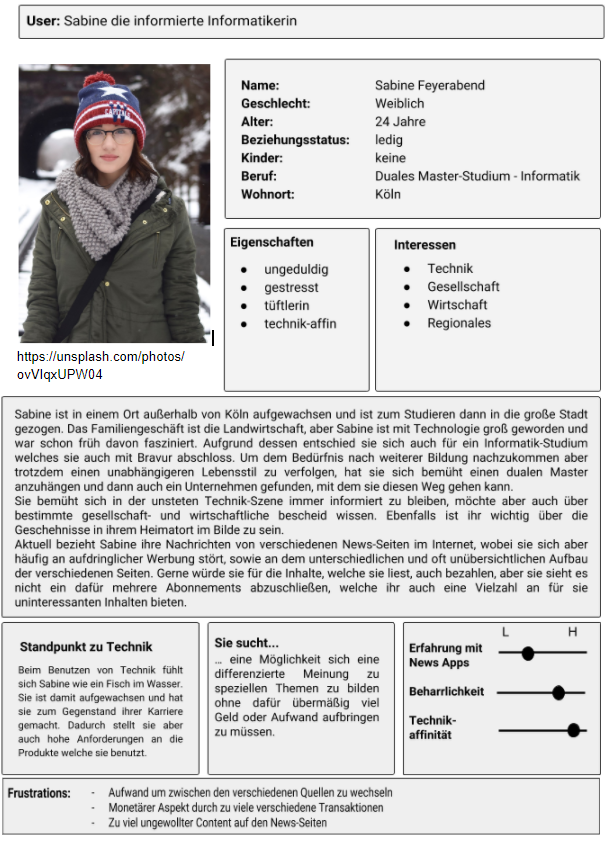
\includegraphics[width=\textwidth-1cm]{persona sabine}
  \caption{Persona 1 - Sabine}
  \label{fig:persona-sabine}
\end{figure}

\clearpage

\begin{figure}[H]
  \centering
  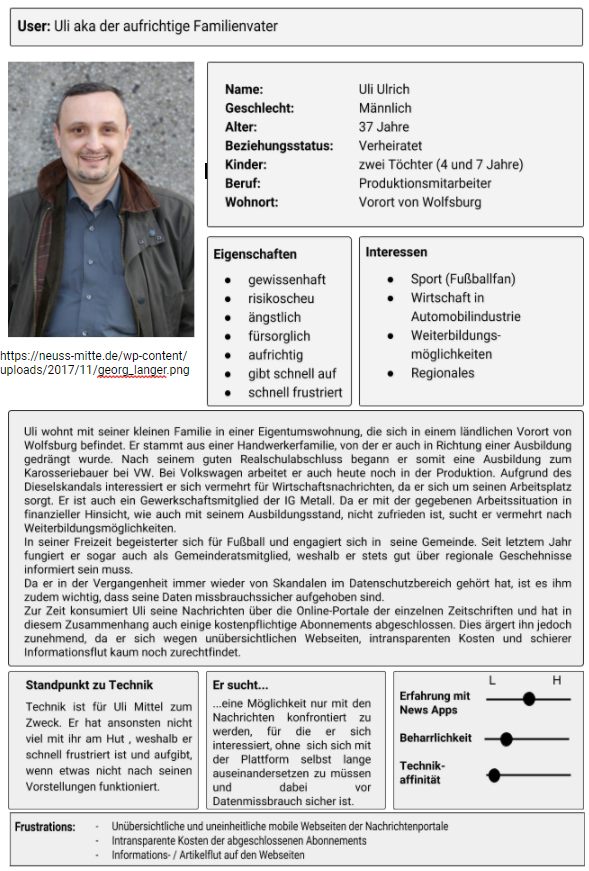
\includegraphics[width=\textwidth-1cm]{persona uli}
  \caption{Persona 2 - Uli}
  \label{fig:persona-uli}
\end{figure}
